\renewcommand*{\arraystretch}{1.1}

\subsection*{Interactive / complex / 4}
\label{section:interactive-complex-read-04}

% change \emph{} to use sans-serif font
\let\oldemph\emph
\renewcommand{\emph}[1]{{\footnotesize \sf #1}}

\renewcommand{\currentQueryCard}{4}
\marginpar{
	\raggedleft
	\vspace{0.22ex}

	\queryRefCard{interactive-complex-read-01}{IC}{1}\\
	\queryRefCard{interactive-complex-read-02}{IC}{2}\\
	\queryRefCard{interactive-complex-read-03}{IC}{3}\\
	\queryRefCard{interactive-complex-read-04}{IC}{4}\\
	\queryRefCard{interactive-complex-read-05}{IC}{5}\\
	\queryRefCard{interactive-complex-read-06}{IC}{6}\\
	\queryRefCard{interactive-complex-read-07}{IC}{7}\\
	\queryRefCard{interactive-complex-read-08}{IC}{8}\\
	\queryRefCard{interactive-complex-read-09}{IC}{9}\\
	\queryRefCard{interactive-complex-read-10}{IC}{10}\\
	\queryRefCard{interactive-complex-read-11}{IC}{11}\\
	\queryRefCard{interactive-complex-read-12}{IC}{12}\\
	\queryRefCard{interactive-complex-read-13}{IC}{13}\\
	\queryRefCard{interactive-complex-read-14}{IC}{14}\\
}


\noindent\begin{tabularx}{\queryCardWidth}{|>{\queryPropertyCell}p{\queryPropertyCellWidth}|X|}
	\hline
	query & Interactive / complex / 4 \\ \hline
%
	title & New topics \\ \hline
%
	pattern & \centering 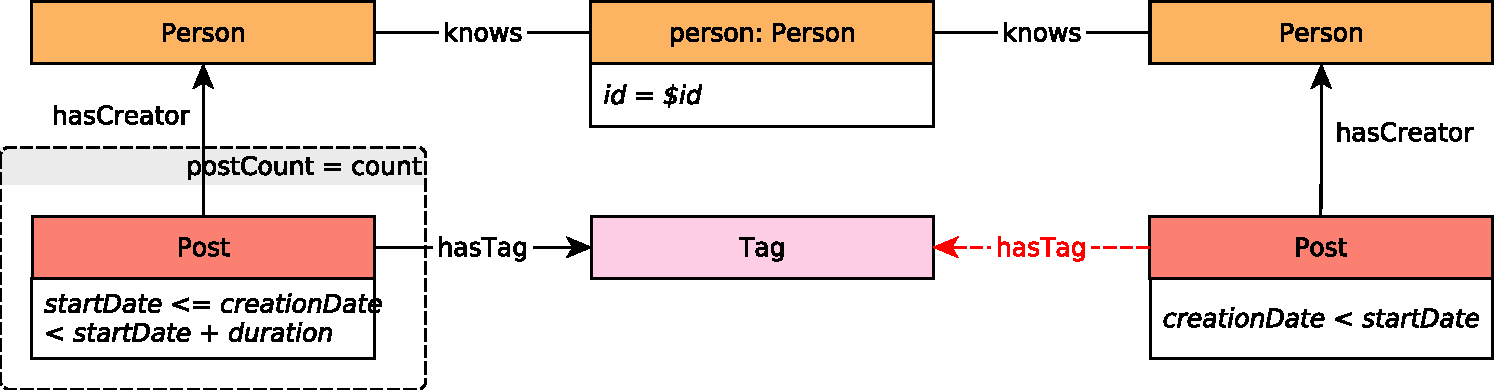
\includegraphics[scale=\patternscale,margin=0cm .2cm]{patterns/interactive-complex-read-04} \tabularnewline \hline
%
	desc. & Given a start \emph{Person} (\texttt{personId}), find \emph{Tags} that
are attached to \emph{Posts} that were created by that \emph{Person}`s
friends. Only include \emph{Tags} that were attached to friends'
\emph{Posts} created within a given time interval, and that were never
attached to friends' \emph{Posts} created before this interval.
 \\ \hline
%
	
		params &
		\innerCardVSpace{\begin{tabularx}{\attributeCardWidth}{|>{\paramNumberCell}c|>{\varNameCell}M|>{\typeCell}m{\typeWidth}|Y|} \hline
		$\mathsf{1}$ & Person.id
 & ID
 & \texttt{personId}
 \\ \hline
		$\mathsf{2}$ & startDate
 & Date
 & \texttt{startDate}
 \\ \hline
		$\mathsf{3}$ & duration
 & 32-bit Integer
 & \texttt{durationDays} -- Duration of requested period, in days. The
interval \texttt{{[}startDate,\ startDate\ +\ duration)} is closed-open
 \\ \hline
		\end{tabularx}}\innerCardVSpace \\ \hline
	
%
	
		result &
		\innerCardVSpace{\begin{tabularx}{\attributeCardWidth}{|>{\resultNumberCell}c|>{\varNameCell}M|>{\typeCell}m{\typeWidth}|>{\resultOriginCell}c|Y|} \hline
		$\mathsf{1}$ & Tag.name & String & R &
				\texttt{tagName}
 \\ \hline
		$\mathsf{2}$ & postCount & 32-bit Integer & A &
				\texttt{postCount} -- Number of Posts made within the given time
interval that have this Tag
 \\ \hline
		\end{tabularx}}\innerCardVSpace \\ \hline
	
%
	
		sort		&
		\innerCardVSpace{\begin{tabularx}{\attributeCardWidth}{|>{\sortNumberCell}c|>{\varNameCell}M|>{\directionCell}c|Y|} \hline
		$\mathsf{1}$ & postCount
 & $\desc
$ &  \\ \hline
		$\mathsf{2}$ & Tag.name
 & $\asc
$ &  \\ \hline
		\end{tabularx}}\innerCardVSpace \\ \hline
	%
	limit & 10 \\ \hline
	%
	CPs &
	\multicolumn{1}{>{\raggedright}l|}{
		\chokePoint{2.3}, 
		\chokePoint{8.2}, 
		\chokePoint{8.5}
		} \\ \hline
	%
	relevance &
		\footnotesize This query looks for paths of length two, starting from a given *Person*, moving to *Posts* and then to *Tags*. It tests the ability of the query optimizer to properly select the usage of hash joins or index based joins, depending on the cardinality of the intermediate results. These cardinalities are clearly affected by the input *Person*, the number of friends, the variety of *Tags*, the time interval and the number of *Posts*.
 \\ \hline%
\end{tabularx}
\queryCardVSpace

% change \emph back to the old one
\let\emph\oldemph